%% Standalone lecture -- build with:  pdflatex -shell-escape introduction
%% Shared preamble for standalone lecture files.
%%
%% Every lecture begins with %% Shared preamble for standalone lecture files.
%%
%% Every lecture begins with %% Shared preamble for standalone lecture files.
%%
%% Every lecture begins with \input{preamble} and is compiled on its own:
%%     pdflatex -shell-escape <lecture>
%% There is no master lectures.tex any more -- the list of lectures lives in
%% lectures.yaml and is read by the build scripts.

\documentclass[25pt,landscape,footrule]{foils}
\input{macros_gen}
\backgroundsetup{contents={}}

\usepackage{stmaryrd}
\usepackage{ifthen}
\usepackage{pdf14}

% figures/ is not duplicated here -- the originals in ../lectures/figures are used
\graphicspath{{figures/}{../lectures/figures/}{~/Documents/figures/}{~/Documents/teaching/courses/comp6208/old_lectures/figures/}{~/Documents/teaching/courses/comp3008/new_lectures/figures/}{~/Documents/teaching/courses/comp6208/new_lectures/figures/}{~/Documents/teaching/courses/MLshort/figures/}{~/Documents/teaching/courses/comp3212/lectures/figures/}{/Users/apb1/Documents/teaching/courses/comp6208/github/lectures/figures}}

\date{}

\newcounter{lessoncnt}
\newcommand{\lesson}[1]{\setcounter{page}{1}%
\section{Mathematics of Machine Learning\\%
\vfill
\textcolor{red}{\textit{#1}}
\vfill}}
 and is compiled on its own:
%%     pdflatex -shell-escape <lecture>
%% There is no master lectures.tex any more -- the list of lectures lives in
%% lectures.yaml and is read by the build scripts.

\documentclass[25pt,landscape,footrule]{foils}
\input{macros_gen}
\backgroundsetup{contents={}}

\usepackage{stmaryrd}
\usepackage{ifthen}
\usepackage{pdf14}

% figures/ is not duplicated here -- the originals in ../lectures/figures are used
\graphicspath{{figures/}{../lectures/figures/}{~/Documents/figures/}{~/Documents/teaching/courses/comp6208/old_lectures/figures/}{~/Documents/teaching/courses/comp3008/new_lectures/figures/}{~/Documents/teaching/courses/comp6208/new_lectures/figures/}{~/Documents/teaching/courses/MLshort/figures/}{~/Documents/teaching/courses/comp3212/lectures/figures/}{/Users/apb1/Documents/teaching/courses/comp6208/github/lectures/figures}}

\date{}

\newcounter{lessoncnt}
\newcommand{\lesson}[1]{\setcounter{page}{1}%
\section{Mathematics of Machine Learning\\%
\vfill
\textcolor{red}{\textit{#1}}
\vfill}}
 and is compiled on its own:
%%     pdflatex -shell-escape <lecture>
%% There is no master lectures.tex any more -- the list of lectures lives in
%% lectures.yaml and is read by the build scripts.

\documentclass[25pt,landscape,footrule]{foils}
\input{macros_gen}
\backgroundsetup{contents={}}

\usepackage{stmaryrd}
\usepackage{ifthen}
\usepackage{pdf14}

% figures/ is not duplicated here -- the originals in ../lectures/figures are used
\graphicspath{{figures/}{../lectures/figures/}{~/Documents/figures/}{~/Documents/teaching/courses/comp6208/old_lectures/figures/}{~/Documents/teaching/courses/comp3008/new_lectures/figures/}{~/Documents/teaching/courses/comp6208/new_lectures/figures/}{~/Documents/teaching/courses/MLshort/figures/}{~/Documents/teaching/courses/comp3212/lectures/figures/}{/Users/apb1/Documents/teaching/courses/comp6208/github/lectures/figures}}

\date{}

\newcounter{lessoncnt}
\newcommand{\lesson}[1]{\setcounter{page}{1}%
\section{Mathematics of Machine Learning\\%
\vfill
\textcolor{red}{\textit{#1}}
\vfill}}


\begin{document}

\lesson{Introduction}
\vspace{-1cm}
\begin{center}
\noindent\includegraphics[height=100mm]{cnn1.jpeg}
\end{center}
\keywords{Course Details and Topics}
%%%%%%%%%%%%%%%%%%%%%%% Next Slide %%%%%%%%%%%%%%%%%%%%%%%
\renewcommand{\Outline}{%
\begin{slide}
\section[1]{Outline}

\begin{minipage}{12cm}\raggedright
  \begin{enumerate}\squeeze
    \outlineitem{Why are you doing this course?}{why}
    \outlineitem{What we assume that you know}{background}
  \end{enumerate}
\end{minipage}\hfill
\begin{minipage}{10cm}
  \includegraphics[width=10cm]{cnn1.jpeg}
\end{minipage}
\end{slide}
\addtocounter{outlineitem}{1}
}

\setcounter{outlineitem}{1}


%%%%%%%%%%%%%%%%%%%%%%% Next Slide %%%%%%%%%%%%%%%%%%%%%%%
\Outline % Outline
\toptarget{firstoutline}
%%%%%%%%%%%%%%%%%%%%%%% Next Slide %%%%%%%%%%%%%%%%%%%%%%%

\begin{slide}
\section{Orientation}

\begin{PauseHighLight}
  \begin{itemize}
  \item This courses addresses three cohorts of students:
    \begin{itemize}
    \item Third year Artificial Intelligence Students
    \item MSc in Machine Learning Students
    \item Volunteers\pause
    \end{itemize}
  \item It is dual coded (AICE3001/AICE6002), with subtle difference
    in expectations reflected in slightly different evaluation\pause
  \item Notes are on Moodle and
    \begin{quote}
      https://ecs-vlc.github.io/aice3001/\pause
    \end{quote}
  \end{itemize}
\end{PauseHighLight}

\end{slide}

%%%%%%%%%%%%%%%%%%%%%%% Next Slide %%%%%%%%%%%%%%%%%%%%%%%

\begin{slide}
  \section{Why are We Teaching You This?}
  
\begin{PauseHighLight}
  \begin{itemize}
  \item In a world where LLMs can do everything, why bother with
    learning mathematics?\pause
  \item You need to learn to trust your own judgement\pauseb
  \item LLMs can help us a lot, but if you don't trust yourself you
    are disempowered\pauseb
  \item This course is aimed at building up trust in your
    understanding of how machine learning works\pauseb
  \end{itemize}
\end{PauseHighLight}

\end{slide}

%%%%%%%%%%%%%%%%%%%%%%% Next Slide %%%%%%%%%%%%%%%%%%%%%%%

\begin{slide}
\section{Why Mathematics?}

\begin{PauseHighLight}
  \begin{itemize}
  \item Learning machines are notoriously difficult to
    understand\pause
  \item Mathematics allows us to reason rigorously\pause
  \item Posing question mathematically and seeking mathematical
    solutions provide allow us to build a strong intuition\pause---we
    can't cheat\pauseb{} that much\pauseb
  \item Mathematics also allow us to describe the world
    precisely\pause
  \item It also provides an arsenal of tools that turn out to be hugely
    useful\pause
  \end{itemize}
\end{PauseHighLight}

\end{slide}

%%%%%%%%%%%%%%%%%%%%%%% Next Slide %%%%%%%%%%%%%%%%%%%%%%%

\begin{slide}
\section{Cracking the Code}

\begin{PauseHighLight}
  \begin{itemize}
  \item Mathematics is a language that takes time to master\pause
  \item For some it is easy, for others it will be a struggle\pause
  \item But given determination everyone can crack the code and
    understand what the mathematics is saying\pause
  \item This comes from engaging and working with maths\pause---this course has
    tutorials that should be considered compulsory\pauseb{} not because
    there are marks attached, but because without doing the work you
    aren't going to crack the code\pauseb
  \end{itemize}
\end{PauseHighLight}

\end{slide}

%%%%%%%%%%%%%%%%%%%%%%% Next Slide %%%%%%%%%%%%%%%%%%%%%%%

\begin{slide}
\section{Starting from Different Places}

\begin{PauseHighLight}
  \begin{itemize}
  \item You all start from different places\pause
  \item Some of you may have a degree in mathematics\pause
  \item For others it may have been you least favourite subject\pause
  \item I invite strong mathematicians to become even
    stronger\pause---the best way to learn is through teaching
    others\pauseb
  \item For students starting from a weak base, judge yourselves by
    your progress, not by comparing yourself to others\pause
  \end{itemize}
\end{PauseHighLight}

\end{slide}

%%%%%%%%%%%%%%%%%%%%%%% Next Slide %%%%%%%%%%%%%%%%%%%%%%%

\begin{slide}
\section{The Golden Rule of Mathematics}

\begin{PauseHighLight}
  \begin{itemize}
  \item \emph{Understand every step}\pause
  \item When you don't understand a step, stop\pause, break the
    problem down\pauseb, ask someone\pauseb
  \item Mathematics uses a lot of short-cuts\pause, which speeds-up
    calculations\pause, but you need to be able to justify every
    step\pauseb
  \item It takes bravery to admit you don't understand and insist that
    you will\pauseb
  \item Asking ``stupid'' questions isn't stupid\pauseb{} it is how we
    all learn\pauseb
  \end{itemize}
\end{PauseHighLight}

\end{slide}

%%%%%%%%%%%%%%%%%%%%%%% Next Slide %%%%%%%%%%%%%%%%%%%%%%%

\begin{slide}
\section{The Journey}

\begin{PauseHighLight}
  \begin{itemize}
  \item We are going to visit lots of aspects of mathematics that have
    proved fruitful in machine learning\pause
  \item Some of this will be very concrete, while in other cases by
    look at a higher level of abstraction we can generalise methods
    across different application areas\pause
  \item We will cover, calculus, vector spaces, convexity,
    optimisation, entropy, probability, statistics and much else
    besides\pause
  \item The journey will pay you off\pause, these are the foundations
    of most of machine learning and will give you super-powers that
    are hard to acquire without mathematics\pause
  \end{itemize}
\end{PauseHighLight}

\end{slide}

%%%%%%%%%%%%%%%%%%%%%%% Next Slide %%%%%%%%%%%%%%%%%%%%%%%
\Outline % What we assume you know?
%%%%%%%%%%%%%%%%%%%%%%% Next Slide %%%%%%%%%%%%%%%%%%%%%%%

\begin{slide}
\section{What we Assume you Know}
  
\begin{PauseHighLight}
  \begin{itemize}
  \item You should all have A-level mathematics and have done some
    mathematics at Uni\pause
  \item You should know what a function is, e.g. $f(x) = x^2+3$\pause
  \item You should be able to do simple algebraic manipulations\pause
  \item And some elementary calculus
    \begin{align*}
      f'(x) = \frac{\dd (x^2+3)}{\dd x} = 2\,x\pause
    \end{align*}
  \end{itemize}
\end{PauseHighLight}

\end{slide}

%%%%%%%%%%%%%%%%%%%%%%% Next Slide %%%%%%%%%%%%%%%%%%%%%%%

\begin{slide}
\section{Vectors}

\begin{PauseHighLight}
  \begin{itemize}
  \item Ordinary vectors (what mathematicians call elements of
    $\mathbb{R}^n$) are much used in machine learning and should be
    familiar\pause
  \item We will use bold symbols to represent \emph{column vectors}, e.g.
    \begin{align*}
      \bm{x} =
      \begin{pmatrix}
        1.2 \\ 2.3 \\ 4.7
      \end{pmatrix}\pause
    \end{align*}
  \item We denote \emph{row vectors} as the \emph{transpose} of column
    vectors $\bm{x}^\tr = (1.2, 2.3, 4.7)$\pause
  \item We care whether vectors are row of column vectors as it allows
    us to write equation involving vectors succinctly and unambiguously\pause
  \end{itemize}
\end{PauseHighLight}

\end{slide}

%%%%%%%%%%%%%%%%%%%%%%% Next Slide %%%%%%%%%%%%%%%%%%%%%%%

\begin{slide}
\section{Matrices}

\begin{PauseHighLight}
  \begin{itemize}
  \item Matrices are blocks of number that define linear mappings
    between vectors, e.g. $\mat{M} \in \mathbb{R}^{2\times3}$ 
    \begin{align*}
      \mat{M} =
      \begin{pmatrix}
        1.1 & -2.1 & 6.2 \\ 9.3 & 3.1 &-4.4
      \end{pmatrix}\pause
    \end{align*}
  \item An $m\times n$ matrix (i.e. $\mat{M} \in \mathbb{R}^{m\times
      n}$) has $m$ rows and $n$ columns\pause
  \item An $m \times n$ matrix acting on a vector in $\mathbb{R}^n$
    transforms it to $\mathbb{R}^m$ vector, e.g.
    \begin{align*}
      \mat{M} \, \bm{x} =
      \begin{pmatrix}
        1.1 & -2.1 & 6.2 \\ 9.3 & 3.1 &-4.4
      \end{pmatrix}
      \begin{pmatrix}
        1.2 \\ 2.3 \\ 4.7\
      \end{pmatrix}
      =
      \begin{pmatrix}
        28.63 \\ -2.39
      \end{pmatrix}\pause
      \end{align*}
  \end{itemize}
\end{PauseHighLight}

\end{slide}

%%%%%%%%%%%%%%%%%%%%%%% Next Slide %%%%%%%%%%%%%%%%%%%%%%%

\begin{slide}
\section{Composition of Mappings}

\begin{PauseHighLight}
  \begin{itemize}
  \item Matrices, $\mat{A}$, $\mat{B}$, etc. represent mappings
    between spaces\pause
  \item Provided the matrices are the correct size we can compose
    these mappings,  e.g. if $\mat{A} \in \mathbb{R}^{\ell \times m}$
    and $\mat{B} \in \mathbb{R}^{m\times n}$ then $\mat{A} \, \mat{B}$
    represents the effect of
    \begin{itemize}
    \item first applying $\mat{B}$ to vectors in $\mathbb{R}^n$ to
      obtain vectors in $\mathbb{R}^m$\pause
    \item and then applying $\mat{A}$ to get vectors in $\mathbb{R}^{\ell}$
    \end{itemize}
    \begin{align*}
      \mat{A}\, \mat{B} \, \bm{x} = \mat{A} \,(\mat{B}\, \bm{x})\pause
    \end{align*}
  \end{itemize}
\end{PauseHighLight}

\end{slide}


%%%%%%%%%%%%%%%%%%%%%%% Next Slide %%%%%%%%%%%%%%%%%%%%%%%

\begin{slide}
\section[-2]{Matrix Multiplication}

\pb
\begin{itemize}
\item The combined mapping $\mat{A}\,\mat{B}$ can be represprested
  by an $\ell \times n$ matrix $\mat{C}$ which we can compute using
  matrix multiplcation (rows times columns)\pause
  \begin{center}
    \multipdf[width=0.9\textwidth]{matrix_multiplication}\pause
  \end{center}
\item Matrix multiplication is associative: $(\mat{A}\,\mat{B})\,\mat{C} = \mat{A}\, (\mat{B}\, \mat{C})$\pause
\item But in general not commutative $\mat{A}\,\mat{B} \neq \mat{B}\, \mat{A}$\pause
\end{itemize}

\end{slide}

%%%%%%%%%%%%%%%%%%%%%%% Next Slide %%%%%%%%%%%%%%%%%%%%%%%

\begin{slide}
\section[-2]{Transpose}

\begin{PauseHighLight}
  \begin{itemize}
  \item We often encounter transposes of a matrix $\mat{M}^\tr$ where
    we have exchanged the rows and columns: $[\mat{M}^\tr]_{ij} =
    [\mat{M}]_{ji}$\pause
  \item Clear $(\mat{M}^\tr)^\tr = \mat{M}$\pause
  \item It is simple question of book keeping to show that
    \begin{align*}
      (\mat{A}\,\mat{B})^\tr &= \mat{B}^\tr \mat{A}^\tr\pause
    \end{align*}
  \item For a symmetric matrix $\mat{M} = \mat{M}^\tr$\pause
  \item Since $1\times 1$ matrices are always symmetric
    \begin{align*}
      \bm{a}^\tr \bm{b} &= (\bm{a}^\tr \bm{b})^\tr = \bm{b}^\tr
                          \bm{a}\pause\\
      \bm{a}^\tr \mat{M} \bm{b} &= \bm{b}^\tr \mat{M}^\tr \bm{a}\pauseb
    \end{align*}
  \end{itemize}
\end{PauseHighLight}

\end{slide}


%%%%%%%%%%%%%%%%%%%%%%% Next Slide %%%%%%%%%%%%%%%%%%%%%%%

\begin{slide}
\section{Matrix-Vector Multiplication}
\pb
\begin{itemize}
\item We can treat a column vector as a $n\times 1$ matrix\pause
\item Then matrix-vector multiplication can be treated the same as
  matrix multiplication\pause
  \begin{center}
    \multipdf[width=0.6\textwidth]{matrix_vector_multiplication}\pause
  \end{center}
  
\end{itemize}

\end{slide}

%%%%%%%%%%%%%%%%%%%%%%% Next Slide %%%%%%%%%%%%%%%%%%%%%%%

\begin{slide}
\section[-1]{Inner Products}

\pb
\begin{itemize}
\item The dot or inner-product between two vectors with the same
  number of elements, can be written $\bm{a}^\tr\bm{b}$\pause
  \begin{center}
    \multipdf[width=0.5\textwidth]{vector_inner_product}\pause
  \end{center}
\item Inner products encode  angles between vectors
  \begin{align*}
    \bm{a}^\tr\bm{b} = \|\bm{a}\| \, \|\bm{b}\| \cos(\theta)\pause
  \end{align*}
\end{itemize}


\end{slide}

%%%%%%%%%%%%%%%%%%%%%%% Next Slide %%%%%%%%%%%%%%%%%%%%%%%

\begin{slide}
\section{Outer Products}

\pb
\begin{itemize}
\item We can also define the outer-produce between any size vectors, $\bm{a}\,\bm{b}^\tr$\pause
  \begin{center}
    \multipdf[width=0.8\textwidth]{vector_outer_product}\pause
  \end{center}
\item Notice that we need to know whether we are dealing with row or
  column vectors\pause
\end{itemize}
\end{slide}

%%%%%%%%%%%%%%%%%%%%%%% Next Slide %%%%%%%%%%%%%%%%%%%%%%%

\begin{slide}
\section[-2]{Norms}

\begin{PauseHighLight}
  \begin{itemize}
  \item Norms are non-negative numbers associated with the ``size'' of
    a vector\pause
  \item The norm you should be familiar with is the \emph{Euclidean
      Norm} or 2-norm
    \begin{align*}
      \|\bm{x}\|_2 = \sqrt{\sum_{i=1}^n x_i^2}\pause = \sqrt{x_1^2 +
      x_2^2 + \ldots + x_n^2}\pauseb = \sqrt{\bm{x}^\tr \bm{x}}\pauseb
    \end{align*}
  \item We will see there exist other norms (using different ways of
    measuring size)\pause
  \item The Euclidean norm is intimately related to the inner-product,
    we will see other examples of this for different vector spaces\pause
  \end{itemize}
\end{PauseHighLight}

\end{slide}

%%%%%%%%%%%%%%%%%%%%%%% Next Slide %%%%%%%%%%%%%%%%%%%%%%%

\begin{slide}
\section[-1]{Matrices as Linear Mappings}

\begin{PauseHighLight}
  \begin{itemize}
  \item Matrices represent mappings between vectors
    \begin{align*}
      \bm{b} = \mat{M}\, \bm{a} 
    \end{align*}
  \item The elements of $\bm{b}$ are \emph{linear sums} of the elements of
    $\bm{a}$
    \begin{align*}
      b_i = \sum_j M_{ij} a_j\pause = M_{i1} a_1 + M_{i2} a_2 + \cdots + M_{in} a_n\pauseb
    \end{align*}
  \item Two important consequences of this linearity are for any real
    $c$
    \begin{align*}
      \mat{M}\, (c\,\bm{a}) &= c\, (\mat{M}\, \bm{a}) \pause\\
      \mat{M} (\bm{a} + \bm{b}) &= (\mat{M}\, \bm{a}) + (\mat{M}\, \bm{b})\pauseb
    \end{align*}
  \end{itemize}
\end{PauseHighLight}

\end{slide}

%%%%%%%%%%%%%%%%%%%%%%% Next Slide %%%%%%%%%%%%%%%%%%%%%%%

\begin{slide}
\section[-2]{Action Of Matrices on Volumes}

\begin{PauseHighLight}
  \begin{itemize}
  \item For a closed set of points corresponding to a
    volume, $V$ in $\mathbb{R}^n$, treating each point as a
    vector, we can as what happens to the volume after mapping the
    vector by a matrix
    \begin{center}
      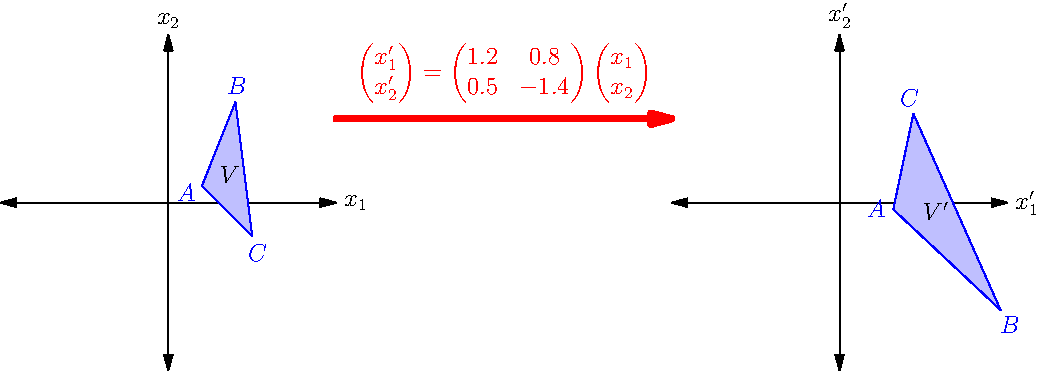
\includegraphics[width=0.8\linewidth]{volume_mapping}\pause
    \end{center}
  \item For square matrices, $\mat{M}$, the determinant is equal to
    $\det(\mat{M}) = \pm V'/V$\pause
  \item The sign tells us if there has been a reflection\pause
  \end{itemize}
\end{PauseHighLight}

\end{slide}

%%%%%%%%%%%%%%%%%%%%%%% Next Slide %%%%%%%%%%%%%%%%%%%%%%%

\begin{slide}
\section{Determinants}

\begin{PauseHighLight}
  \begin{itemize}
  \item A consequence of the fact that $\mat{A}\,\mat{B}$ denotes the
    composition, apply mapping $\mat{B}$ then apply mapping $\mat{A}$
    \begin{align*}
      \det(\mat{A}\,\mat{B}) = \det(\mat{A}) \times \det(\mat{B})\pause
    \end{align*}
  \item Determinants are only defined for square matrices, as
    non-square matrices project into different size spaces, where the
    volumes cannot be compared\pause
  \item \emph{Singular matrices} projects all points onto a lower
    dimensional space, so have determinant 0\pause
  \end{itemize}
\end{PauseHighLight}

\end{slide}



%%%%%%%%%%%%%%%%%%%%%%% Next Slide %%%%%%%%%%%%%%%%%%%%%%%

\begin{slide}
\section{Multivariate Functions}

\begin{PauseHighLight}
  \begin{itemize}
  \item In machine learning we heavily use multivariate functions
    $f:\mathbb{R}^n \rightarrow \mathbb{R}^m$\pause
  \item Often our functions will be scalared value $f:\mathbb{R}^n
    \rightarrow \mathbb{R}$\pause
  \item E.g. a learning machine for regression might be
    $\hat{f}(\bm{x}, \bm{w})$\pause{} or we might have a loss function $L(\bm{w})$\pauseb
  \item We say a function $f$ is linear if
    \begin{align*}
      f(c\, \bm{x}) &= c\, f(\bm{x}) & f(\bm{x}+\bm{y}) = f(\bm{x}) +
                                       f(\bm{y})\pause
    \end{align*}
  \end{itemize}
\end{PauseHighLight}

\end{slide}

%%%%%%%%%%%%%%%%%%%%%%% Next Slide %%%%%%%%%%%%%%%%%%%%%%%

\begin{slide}
\section{Gradients}

\begin{PauseHighLight}
  \begin{itemize}
  \item The gradient of a function $f:\mathbb{R}^n
    \rightarrow \mathbb{R}$ at a point $\bm{x}^*$ is define as the
    column vector
    \begin{align*}
      \grad f(\bm{x}) =
      \begin{pmatrix}
        \pd{f(\bm{x}^*)}{x_1} \\
        \pd{f(\bm{x}^*)}{x_2} \\
        \vdots \\
        \pd{f(\bm{x})^*}{x_n}
      \end{pmatrix}\pause
    \end{align*}
  \item The gradient vector is orthogonal to the contour plane and
    points in the direction that the function increases in fastest\pause 
  \end{itemize}
\end{PauseHighLight}

\end{slide}


%%%%%%%%%%%%%%%%%%%%%%% Next Slide %%%%%%%%%%%%%%%%%%%%%%%

\begin{slide}
\section{Probability}

\begin{PauseHighLight}
  \begin{itemize}
  \item We will have a lot to say about probability later in this course\pause
  \item To reason about events with uncertain outcomes we introduce
    \emph{random variables}\pause
  \item Random variables corresponds to objects that we assign numbers
    to depending on the outcome of a random event\pause
  \item E.g. we might assign 0 to the outcome of tossing a tail and 1
    for a head\pause{}---this is an example of a discrete random variable\pauseb
  \item A continuous random variable might be the temperature at 12
    noon tomorrow in Hyde park\pauseb
  \end{itemize}
\end{PauseHighLight}

\end{slide}

%%%%%%%%%%%%%%%%%%%%%%% Next Slide %%%%%%%%%%%%%%%%%%%%%%%

\begin{slide}
\section{Probability Distributions}

\begin{PauseHighLight}
  \begin{itemize}
  \item For discrete events, we can define a \emph{probability mass
      function} $\Prob{X=x}$ that the random variable takes the value
    $x$\pause
  \item This is a number between 0 and 1 with
    $\sum_{x\in\mathcal{X}}\Prob{X=x} =1$\pause
  \item For continuous events the probability of $X$ taking a
    particular value $x$ is zero\pause
  \item Instead we consider the probability density $f_X(x)$ which we
    can define as
    \begin{align*}
      f_X(x) = \lim_{\delta x \rightarrow 0} \frac{\Prob{x<X\leq
      x+\delta x}}{\delta x}\pause
    \end{align*}
  \end{itemize}
\end{PauseHighLight}


\end{slide}

%%%%%%%%%%%%%%%%%%%%%%% Next Slide %%%%%%%%%%%%%%%%%%%%%%%

\begin{slide}
\section[-2]{Expectations}

\begin{PauseHighLight}
  \begin{itemize}
  \item One of the most useful quantities in dealing with random
    numbers is to look at the average value, aka as the
    \emph{expectation}, for some function $g(X)$ of the random variable
    \begin{align*}
      \av{g(X)} =
      \begin{cases}
        \sum_{x\in \mathcal{X}} \Prob{X=x} \, g(x) \\
        \int f_X(x) \, g(x) \, \dd x
      \end{cases}\pause
    \end{align*}
  \item Expectations are linear operators
    \begin{align*}
      \av{c\, g(X)} &= c\, \av{g(x)} \\ \av{g(X) + h(X)} &= \av{g(X)} + \av{h(X)}\pause
    \end{align*}
  \item The expectation of a constant is itself $\av{c} = c$ \pause
  \end{itemize}
\end{PauseHighLight}

\end{slide}

%%%%%%%%%%%%%%%%%%%%%%% Next Slide %%%%%%%%%%%%%%%%%%%%%%%

\begin{slide}
\section{Lesson}

\begin{PauseHighLight}
  \begin{itemize}
  \item I've covered material that we assume you know\pause
  \item If you don't, you are going to struggle following any machine
    learning course, so grab a maths book and revise this\pause
  \item We will revisit most of these topics to gain a better
    understanding, but you will be lost in the other machine learning
    modules if you are not familiar with everything I've covered\pause
  \item There are exercises we will go through in the tutorial session
    where you can test your proficiency\pause
  \end{itemize}
\end{PauseHighLight}

\end{slide}

%%% Local Variables:
%%% TeX-master: "lectures"
%%% End:

\end{document}
